%%%%%%%%%%%%%%%%%%%%% chapter.tex %%%%%%%%%%%%%%%%%%%%%%%%%%%%%%%%%
%
% sample chapter
%
% Use this file as a template for your own input.
%
%%%%%%%%%%%%%%%%%%%%%%%% Springer-Verlag %%%%%%%%%%%%%%%%%%%%%%%%%%
%\motto{Use the template \emph{chapter.tex} to style the various elements of your chapter content.}
\chapter{Appendix: Statistical Review}
\label{StatisticalReview} % Always give a unique label
% use \chaptermark{}
% to alter or adjust the chapter heading in the running head

%\abstract*{Each chapter should be preceded by an abstract (10--15 lines long) that summarizes the content. The abstract will appear \textit{online} at \url{www.SpringerLink.com} and be available with unrestricted access. This allows unregistered users to read the abstract as a teaser for the complete chapter. As a general rule the abstracts will not appear in the printed version of your book unless it is the style of your particular book or that of the series to which your book belongs.
%Please use the 'starred' version of the new Springer \texttt{abstract} command for typesetting the text of the online abstracts (cf. source file of this chapter template \texttt{abstract}) and include them with the source files of your manuscript. Use the plain \texttt{abstract} command if the abstract is also to appear in the printed version of the book.}

%\abstract{Each chapter should be preceded by an abstract (10--15 lines long) that summarizes the content. The abstract will appear \textit{online} at \url{www.SpringerLink.com} and be available with unrestricted access. This allows unregistered users to read the abstract as a teaser for the complete chapter. As a general rule the abstracts will not appear in the printed version of your book unless it is the style of your particular book or that of the series to which your book belongs.\newline\indent
%Please use the 'starred' version of the new Springer \texttt{abstract} command for typesetting the text of the online abstracts (cf. source file of this chapter template \texttt{abstract}) and include them with the source files of your manuscript. Use the plain \texttt{abstract} command if the abstract is also to appear in the printed version of the book.}

\section{Change of Random Variable}
\label{sec:1}
Let's consider we know the probability of a r.v. $X$, $\px$, and we now want to compute the probability density function of some variable $Y=f(X)$, that is, we need to calculate $\py$.

To understand how this new distribution or {\bf change of random variable} is calculated, let's firstly solve a particular case:

\begin{itemize}
\item $X$ is a uniform distribution in the interval $(0,1)$.


\begin{center}
\begin{tabular}{m{.5\textwidth}m{.4\textwidth}}
 \begin{equation} 
\px = \begin{cases}
1 & {\rm if} \quad 0<x<1\\
0 & {\rm otherwise} 
\end{cases} \nonumber
\end{equation} & 
\raisebox{-8ex}{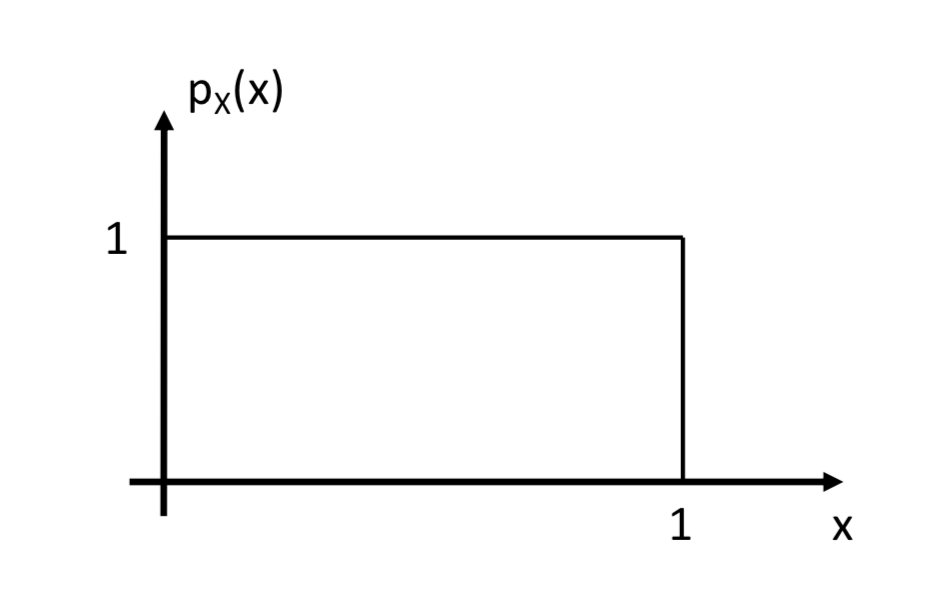
\includegraphics[scale=.25]{Figures/Fig11.png}} \\ 
\end{tabular}
\end{center}

\item $ Y = X^2$. Note that this change produces this transformation:
\begin{center}
\begin{tabular}{m{.5\textwidth}m{.4\textwidth}}
 \raisebox{-8ex}{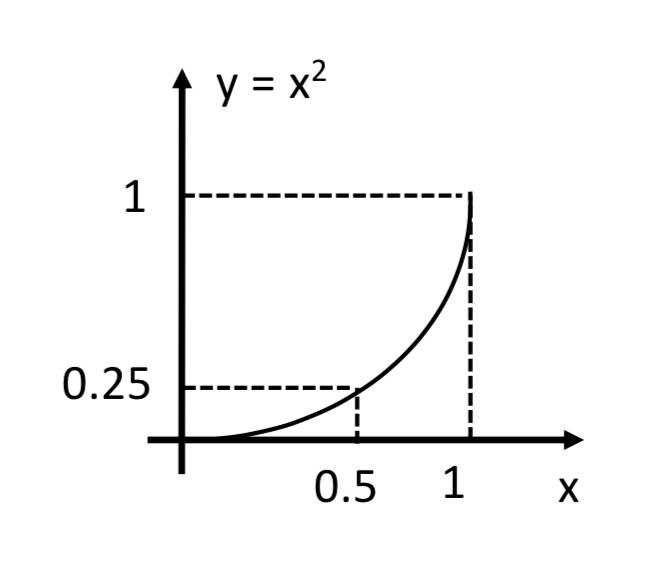
\includegraphics[scale=.4]{Figures/Fig12.png}} &
 \begin{tabular}{l|l}
$x$ & $y = x^2$ \\ \hline
0.1 & 0.01\\
0.2 & 0.04\\
0.5 & 0.25\\
... & ...\\
\end{tabular} 
\end{tabular}
\end{center}

The transformation function $f(\cdot)$ is strictly increasing. So there exists its inverse function $f^{-1}(\cdot)$.


\end{itemize}
To solve this change of r.v., we are going to use the fact that:

\begin{eqnarray}
P\{0<X<0.1\} &  = & P\{0<Y<0.01\}  \nonumber\\
P\{0<X<0.2\} &  = & P\{0<Y<0.04\}  \nonumber\\
P\{0<X<0.5\} &  = & P\{0<Y<0.25\}  \nonumber
\end{eqnarray}
or, in a general case, for any value of $X$, $x_0$, we have
$$ P\{0<X<x_0\}  = P\{0<Y<y_0\}$$
where $y_0=x_0^2$ or $x_0= \sqrt{y_0}$ 

So, we can compute the cumulative distribution function of the r.v. $Y$ as
$$ F_Y(y_0) =  P\{Y<y_0\} =  P\{X<\sqrt{y_0}\}$$

Now, as the cumulative function of $Y$ is expressed in terms of the r.v $X$, we can compute it!!!
\begin{eqnarray} 
F_Y(y_0) =  P\{X<\sqrt{y_0}\} = \int_{-\infty}^{\sqrt{y_0}} \px dx = 
\begin{cases}
\int_{-\infty}^{\sqrt{y_0}} 0 dx = 0 & \quad {\rm if} \quad y_0 <0 \\[2ex]
\int_0^{\sqrt{y_0}} 1 dx = \sqrt{y_0} & \quad {\rm if} \quad 0< y_0 <1 \\[2ex]
\int_0^{1} 1 dx = 1 & \quad {\rm if} \quad y_0 >1 \\
\end{cases}  \nonumber
\end{eqnarray}

So, we have that


\begin{eqnarray} 
F_Y(y_0) =\begin{cases}
 0 & \quad {\rm if} \quad y_0 <0 \\
 \sqrt{y_0} & \quad {\rm if} \quad 0< y_0 <1 \\
 1 & \quad {\rm if} \quad y_0 >1 \\
\end{cases}  \nonumber
\end{eqnarray} 
\begin{center}
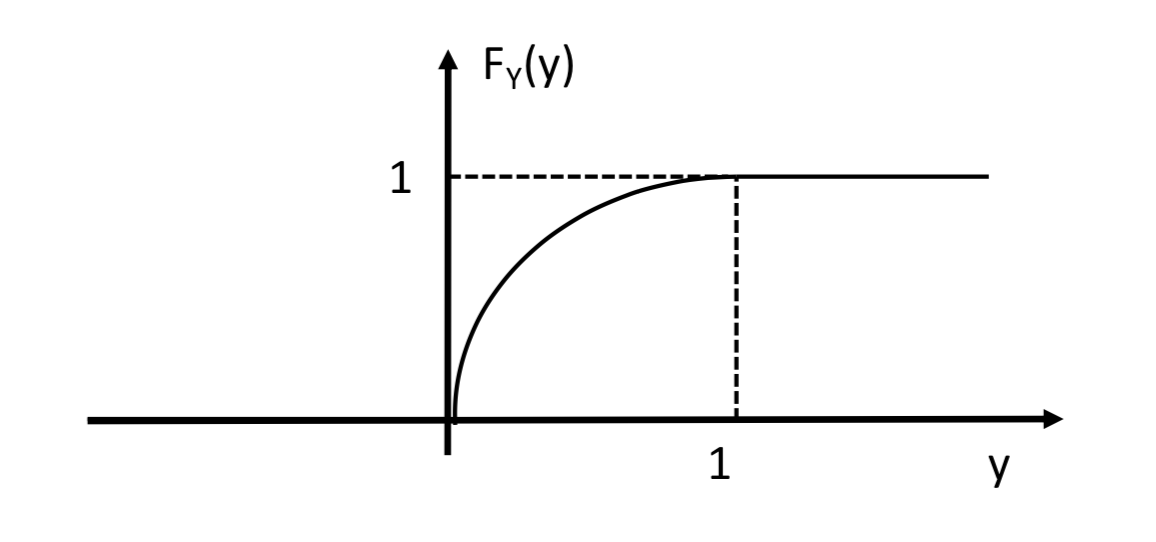
\includegraphics[scale=.4]{Figures/Fig13.png}
\end{center}
and, finally, we can obtain the density function of $Y$ as
\begin{eqnarray} 
\py = \frac{d F_Y(y)}{dy} =\begin{cases}
 \frac{1}{2\sqrt{y}} & \quad {\rm if} \quad 0<y<1 \\
 0 & \quad {\rm otherwise}  \\
\end{cases}  \nonumber
\end{eqnarray} 
\begin{center}
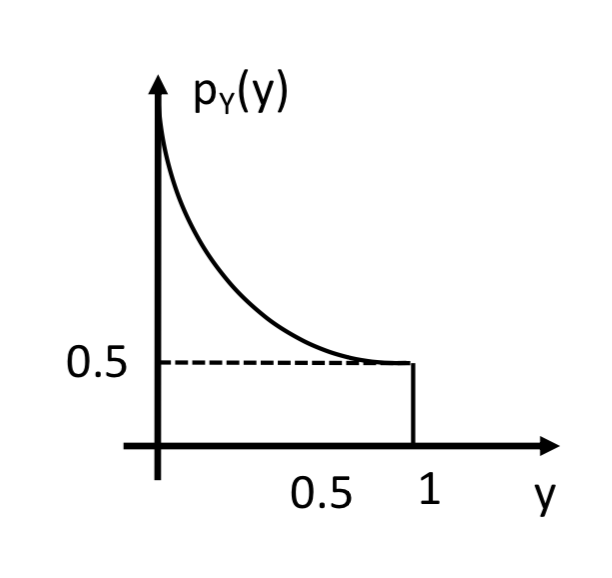
\includegraphics[scale=.4]{Figures/Fig14.png}
\end{center}
Now, let's try to generalize this procedure for any transformation
$$ Y = f(X) $$
being $f(\cdot)$ a strictly increasing function, so $f^{-1}(\cdot)$ exists.
\begin{enumerate}
    \item Compute the cumulative function of $Y$ (by means of $X$)
    \begin{eqnarray} 
    F_Y(y)  &= &  P\{Y<y\} =  P\{X<f^{-1}(y)\} = \int_{-\infty}^{f^{-1}(y)} \px dx = \nonumber \\ 
    & & F_X(f^{-1}(y)) - F_X(-\infty) = F_X(f^{-1}(y)) \nonumber
    \end{eqnarray} 
  Note: $F_X(-\infty) = 0$ for any cumulative distribution function  
    \item Compute the density distribution function (use the chain rule)
    \begin{eqnarray} 
    \py = \frac{d F_Y(y)}{dy} =  \frac{d F_X(f^{-1}(y))}{dy} = \frac{d F_X(x= f^{-1}(y))}{dx}  \frac{dx}{dy} = p_X(x= f^{-1}(y)) \frac{dx}{dy} \nonumber
    \end{eqnarray} 
    So, we obtain that 
    \begin{eqnarray}  \py = p_X(x= f^{-1}(y)) \frac{dx}{dy}  \nonumber \end{eqnarray} 
\end{enumerate}

This formula for the r.v. change can be generalized for any transformation function $f(\cdot)$ which is monotic (either strictly increasing or decreasing) as follows:
\begin{svgraybox}
\begin{eqnarray} 
\py = p_X(x = f^{-1}(y))  \left| \frac{dx}{dy}\right| \label{eq:changeRV}
\end{eqnarray} 
\end{svgraybox}

In fact, we can now use this formula over the previous example:
\begin{center}
\begin{tabular}{m{.2\textwidth}m{.5\textwidth}}
 \raisebox{-0.25ex}{$ Y = X^2$} &
 \begin{equation} 
\px = \begin{cases}
1 & {\rm if} \quad 0<x<1\\
0 & {\rm otherwise} 
\end{cases} \nonumber
\end{equation}
\end{tabular}
\end{center}



each term of the formula \eqref{eq:changeRV} is given by:
\begin{eqnarray} 
\left| \frac{dx}{dy}\right| = \left| \frac{df^{-1}(y)}{dy}\right| = \left| \frac{d\sqrt{y}}{dy}\right| = \frac{1}{2\sqrt{y}} \nonumber
\end{eqnarray} 

\begin{eqnarray} 
p_X(x = f^{-1}(y)) = p_X(x = \sqrt{y}) = \begin{cases}
1 & {\rm if} \quad 0<\sqrt{y}<1\\
0 & {\rm otherwise} 
\end{cases}  \nonumber
\end{eqnarray} 

So, we get

\begin{eqnarray} 
\py  = \frac{1}{2\sqrt{y}} p_X(x = \sqrt{y}) = \begin{cases}
\frac{1}{2\sqrt{y}} & {\rm if} \quad 0<y<1\\
0 & {\rm otherwise} 
\end{cases}  \nonumber
\end{eqnarray} 

In case the transformation function is not monotic, we have to divide the transformation into intervals where we get monotic transformations. That is, we have $Y = f(X)$ and $f(\cdot)$ is not monotic, then redefine the transformation as
\begin{eqnarray} 
Y = \begin{cases} 
f_1(X) & {\rm if } x_0 < x <x_1 \\
f_2(X) & {\rm if } x_1 < x <x_2 \\
\ldots  &  \\
f_N(X) & {\rm if } x_{N-1} < x <x_N \\
\end{cases}  \nonumber
\end{eqnarray}

where $f_1(\cdot),\ldots, f_N(\cdot) $ are monotic. Then, you can compute $\py$ as:
\begin{eqnarray} 
\py =  \sum_{n=1}^N p_X(x = f_n^{-1}(y))  \left| \frac{df_n^{-1}(y)}{dy}\right| \nonumber
\end{eqnarray} 

\subsection{Some usual r.v. changes}

The demonstration of these changes is left as homework.

\begin{enumerate}
    \item SHIFTING of R.V. \\
    $ Y = X+a$, where $a$ is a known constant. Then,
    $$ \py =  p_X(x = y-a) $$
    when we are adding a constant to any r.v., we are shifting the distribution from the origin to the position of the constant
    
    \begin{center}
    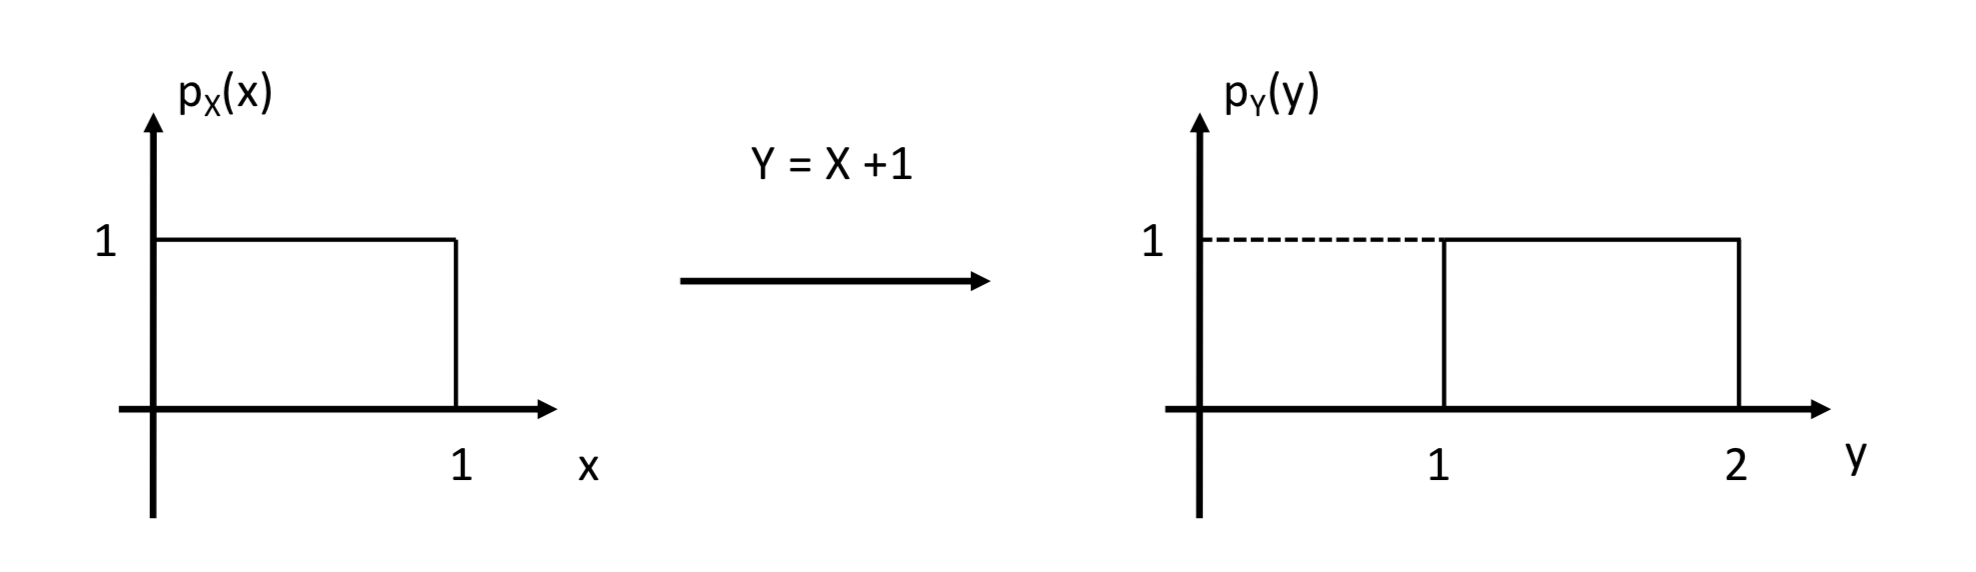
\includegraphics[scale=.3]{Figures/Fig15.png}
    \end{center}
    
    
    \item RESCALING of R.V.\\
    $ Y = aX$, where $a$ is a known constant. Then,
    $$ \py =  \frac{1}{a} p_X(x = \frac{y}{a}) $$
    in this case we are modifying both the support of the distribution function and its height.
    
    \begin{center}
    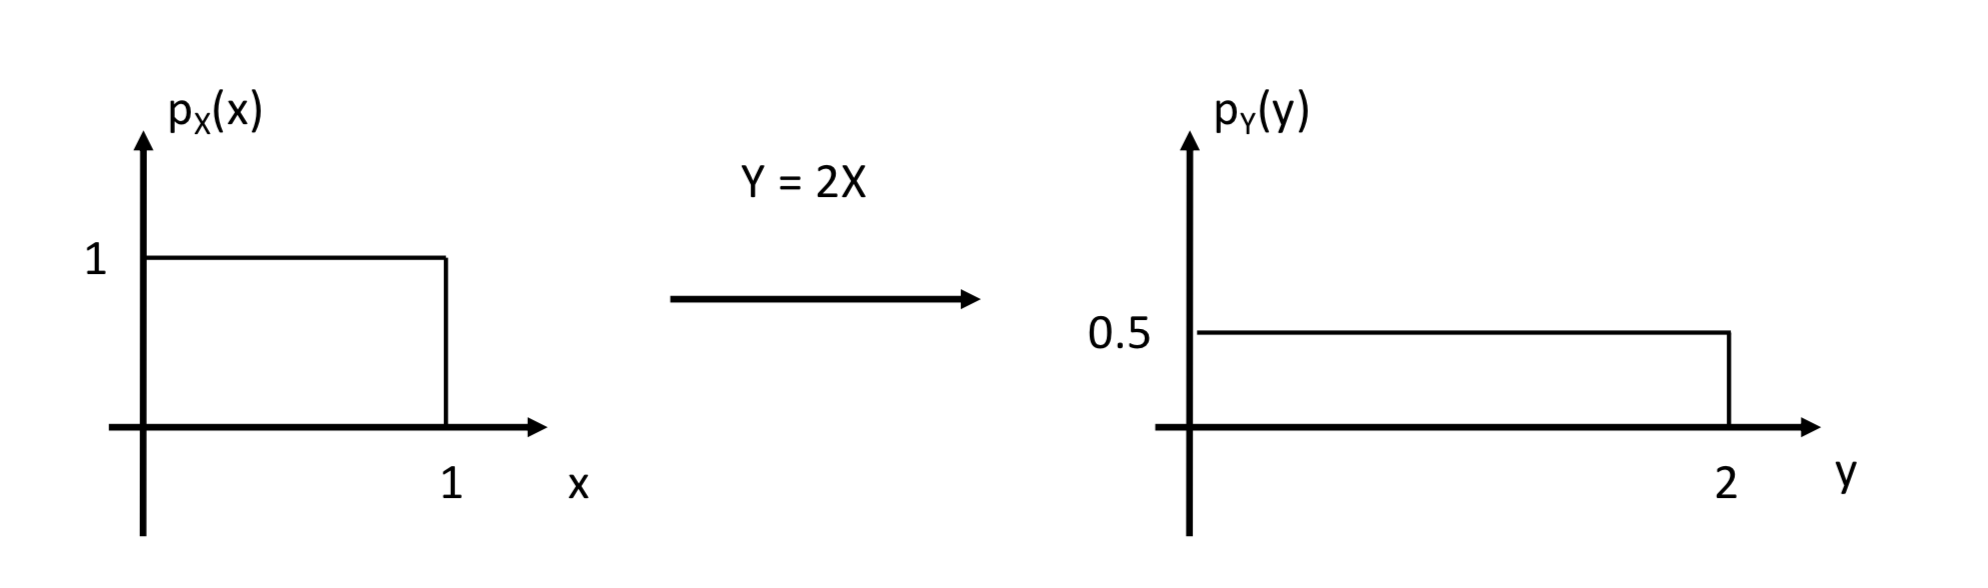
\includegraphics[scale=.3]{Figures/Fig16.png}
    \end{center}
    
\end{enumerate}

